\documentclass[tikz,border=2pt]{standalone}

\usepackage{amsmath,amssymb}
\usepackage{times}
\usetikzlibrary{arrows.meta,calc}

\definecolor{navy}{HTML}{17365D}
\definecolor{voorange}{HTML}{D55E00}
\definecolor{safe}{HTML}{009E73}
\definecolor{cyanblue}{HTML}{56B4E9}
\definecolor{ink}{HTML}{20252B}
\definecolor{midgray}{HTML}{737B83}
\definecolor{lightgray}{HTML}{D9DEE3}

\begin{document}
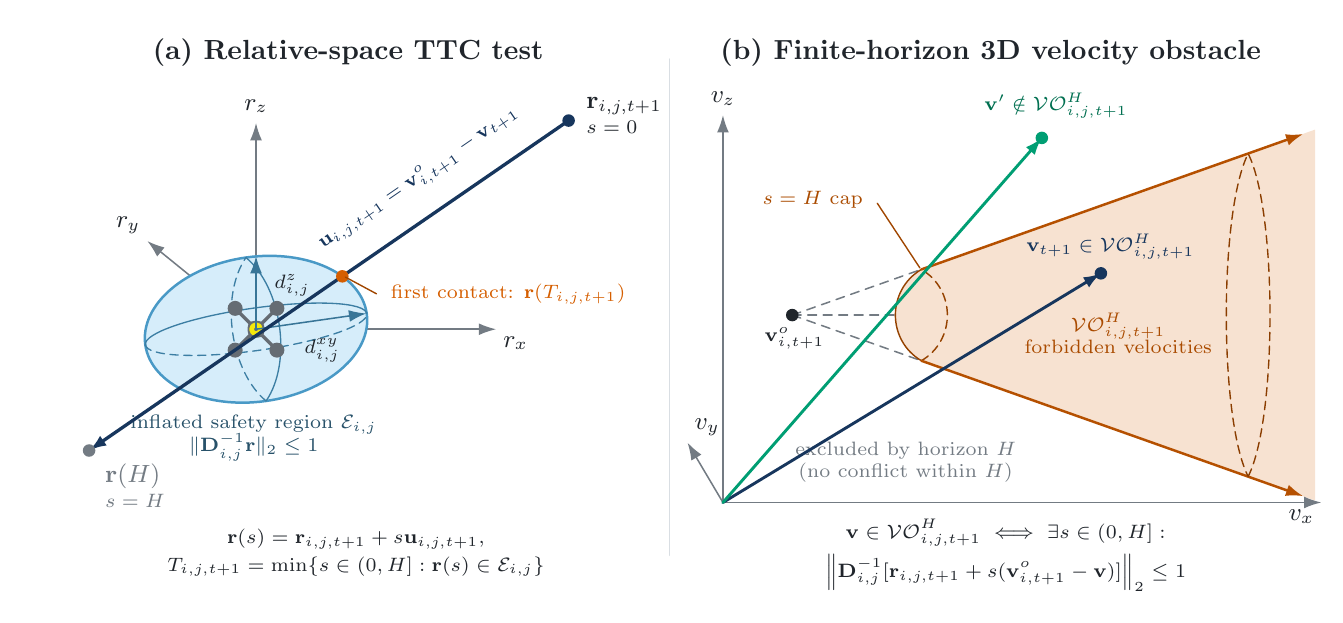
\begin{tikzpicture}[
  x=1cm,
  y=1cm,
  line cap=round,
  line join=round,
  >={Latex[length=2.2mm,width=1.5mm]},
  every node/.style={font=\small, text=ink},
  axis/.style={->, draw=midgray, line width=0.55pt},
  guide/.style={draw=midgray, dash pattern=on 3.2pt off 2.4pt, line width=0.55pt},
  vector/.style={->, draw=navy, line width=1.2pt},
  point/.style={circle, inner sep=1.6pt}
]
  \path[use as bounding box] (-0.15,-0.25) rectangle (16.20,6.95);

  % Panel divider and headings.
  \draw[lightgray, line width=0.65pt] (8.0,0.25) -- (8.0,6.55);
  \node[font=\bfseries] at (3.92,6.64)
    {(a) Relative-space TTC test};
  \node[font=\bfseries] at (12.08,6.64)
    {(b) Finite-horizon 3D velocity obstacle};

  % --------------------------------------------------------------------------
  % Panel (a): anisotropic inflated region and relative trajectory.
  % --------------------------------------------------------------------------
  \coordinate (C) at (2.75,3.12);

  % Oblique 3-D coordinate frame.
  \draw[axis] (C) -- ++(3.05,0) node[below right=-1pt] {$r_x$};
  \draw[axis] (C) -- ++(-1.38,1.12) node[above left=-1pt] {$r_y$};
  \draw[axis] (C) -- ++(0,2.62) node[above] {$r_z$};

  % Anisotropically inflated collision region for one retained primitive.
  \begin{scope}[shift={(C)}, rotate=8]
    \fill[cyanblue!24] (0,0) ellipse (1.42 and 0.92);
    \draw[cyanblue!85!black, line width=0.9pt] (0,0) ellipse (1.42 and 0.92);
    \draw[cyanblue!70!black, densely dashed, line width=0.48pt]
      (-1.42,0) arc[start angle=180,end angle=360,x radius=1.42,y radius=0.27];
    \draw[cyanblue!70!black, line width=0.48pt]
      (1.42,0) arc[start angle=0,end angle=180,x radius=1.42,y radius=0.27];
    \draw[cyanblue!70!black, densely dashed, line width=0.48pt]
      (0,-0.92) .. controls (-0.40,-0.48) and (-0.40,0.48) .. (0,0.92);
    \draw[cyanblue!70!black, line width=0.48pt]
      (0,-0.92) .. controls (0.40,-0.48) and (0.40,0.48) .. (0,0.92);
  \end{scope}

  % Top-view UAV at the origin of the UAV-centered relative-position frame.
  % Drawn directly in TikZ so the standalone PDF remains fully vectorial.
  \begin{scope}[shift={(C)}, scale=0.34]
    \draw[midgray!88!black, line width=1.25pt]
      (-0.22, 0.22) -- (-0.72, 0.72)
      ( 0.22, 0.22) -- ( 0.72, 0.72)
      (-0.22,-0.22) -- (-0.72,-0.72)
      ( 0.22,-0.22) -- ( 0.72,-0.72);
    \fill[midgray!88!black, rounded corners=0.08cm]
      (-0.31,-0.31) rectangle (0.31,0.31);
    \fill[midgray!88!black] (-0.78, 0.78) circle (0.28);
    \fill[midgray!88!black] ( 0.78, 0.78) circle (0.28);
    \fill[midgray!88!black] (-0.78,-0.78) circle (0.28);
    \fill[midgray!88!black] ( 0.78,-0.78) circle (0.28);
    \draw[yellow!95!black, line width=1.7pt] (0,0) circle (0.17);
  \end{scope}

  \node[align=center, font=\scriptsize, cyanblue!45!black]
    at (2.72,1.74)
    {inflated safety region $\mathcal E_{i,j}$\\[-1pt]
     $\|\mathbf D_{i,j}^{-1}\mathbf r\|_2\leq 1$};

  % Safety semiaxes, measured from the ellipsoid center to its boundary.
  \draw[->, draw=cyanblue!65!black, line width=0.55pt]
    (C) -- ($(C)+(1.40,0.20)$)
    node[pos=0.60, below=3pt, font=\scriptsize] {$d^{xy}_{i,j}$};
  \draw[->, draw=cyanblue!65!black, line width=0.55pt]
    (C) -- ($(C)+(0,0.93)$)
    node[pos=0.60, right=3pt, font=\scriptsize] {$d^{z}_{i,j}$};

  % Relative trajectory under constant relative velocity.
  \coordinate (Rzero) at (6.72,5.77);
  % First intersection of the trajectory with the rotated safety ellipse.
  \coordinate (Rttc) at (3.846,3.792);
  \coordinate (Rh) at (0.63,1.58);
  \draw[vector] (Rzero) -- (Rh);
  \node[point, fill=navy] at (Rzero) {};
  \node[point, fill=voorange] at (Rttc) {};
  \node[point, fill=midgray] at (Rh) {};

  \node[anchor=west, align=left] at ($(Rzero)+(0.10,0.06)$)
    {$\mathbf r_{i,j,t+1}$\\[-2pt]\scriptsize $s=0$};
  \draw[voorange!75!black, line width=0.5pt]
    ($(Rttc)+(0.04,-0.01)$) -- (4.28,3.57);
  \node[anchor=west, voorange, font=\scriptsize]
    at (4.34,3.57)
    {first contact: $\mathbf r(T_{i,j,t+1})$};
  \node[anchor=north west, midgray, align=left]
    at ($(Rh)+(0.08,-0.05)$)
    {$\mathbf r(H)$\\[-2pt]\scriptsize $s=H$};
  \node[navy, rotate=34.5, inner sep=0.8pt, font=\scriptsize]
    at (4.82,5.03)
    {$\mathbf u_{i,j,t+1}=\mathbf v^o_{i,t+1}-\mathbf v_{t+1}$};

  \node[font=\scriptsize, align=center] at (4.02,0.28)
    {$\begin{gathered}
      \mathbf r(s)=\mathbf r_{i,j,t+1}+s\mathbf u_{i,j,t+1},\\[-1pt]
      T_{i,j,t+1}=\min\{s\in(0,H]:\mathbf r(s)\in\mathcal E_{i,j}\}
    \end{gathered}$};

  % --------------------------------------------------------------------------
  % Panel (b): conceptual finite-horizon VO in absolute velocity space.
  % --------------------------------------------------------------------------
  \coordinate (Ov) at (8.68,0.92);
  \coordinate (Apex) at (9.56,3.30);
  \coordinate (CapU) at (11.20,3.88);
  \coordinate (CapL) at (11.20,2.72);
  \coordinate (SliceU) at (15.35,5.35);
  \coordinate (SliceL) at (15.35,1.25);
  \coordinate (OpenU) at (16.55,5.78);
  \coordinate (OpenL) at (16.55,0.82);

  % Velocity axes.
  \draw[axis] (Ov) -- ++(-0.45,0.76) node[above right=-1pt] {$v_y$};
  \draw[axis] (Ov) -- ++(0,4.92) node[above] {$v_z$};

  % Infinite-cone guides and finite-horizon cap.
  \draw[guide] (Apex) -- (CapU);
  \draw[guide] (Apex) -- (CapL);
  \draw[guide] (Apex) -- (11.20,3.30);

  % The finite-horizon VO starts at the s=H cap and remains unbounded.
  \begin{scope}
    \clip (10.55,0.72) rectangle (16.20,6.05);
    \path[fill=voorange!18]
      (CapU) -- (OpenU) -- (OpenL) -- (CapL)
      .. controls (10.76,2.98) and (10.76,3.62) .. (CapU)
      -- cycle;
  \end{scope}
  \draw[voorange!70!black, densely dashed, line width=0.52pt]
    (CapL) .. controls (11.64,2.98) and (11.64,3.62) .. (CapU);
  \draw[voorange!70!black, line width=0.52pt]
    (CapU) .. controls (10.76,3.62) and (10.76,2.98) .. (CapL);
  \draw[->, voorange!85!black, line width=0.9pt]
    (CapU) -- (16.05,5.60);
  \draw[->, voorange!85!black, line width=0.9pt]
    (CapL) -- (16.05,1.00);
  \draw[voorange!65!black, densely dashed, line width=0.5pt]
    (SliceL) .. controls (15.72,1.98) and (15.72,4.62) .. (SliceU)
    .. controls (14.98,4.62) and (14.98,1.98) .. (SliceL);

  % Keep the horizontal axis visible beyond the clipped open end of the VO.
  \draw[axis] (Ov) -- (16.28,0.92) node[below left=-1pt] {$v_x$};

  % Apex is the obstacle velocity; the dashed apex-side volume is excluded by H.
  \node[point, fill=ink] at (Apex) {};
  \node[anchor=north, inner sep=1.0pt, font=\scriptsize]
    at ($(Apex)+(0.03,-0.11)$) {$\mathbf v^o_{i,t+1}$};
  \node[font=\scriptsize, midgray, align=center] at (11.00,1.43)
    {excluded by horizon $H$\\(no conflict within $H$)};
  \node[font=\scriptsize, voorange!80!black, align=center]
    at (13.70,3.07)
    {$\mathcal{VO}^{H}_{i,j,t+1}$\\forbidden velocities};
  \draw[voorange!75!black, line width=0.5pt]
    ($(CapU)+(-0.02,0.02)$) -- (10.64,4.72);
  \node[font=\scriptsize, voorange!80!black, anchor=east]
    at (10.58,4.77) {$s=H$ cap};

  % Realized conflicting velocity and a non-conflicting comparison velocity.
  \coordinate (Vin) at (13.48,3.83);
  \coordinate (Vout) at (12.73,5.55);
  \draw[->, draw=navy, line width=1.05pt] (Ov) -- (Vin);
  \node[point, fill=navy] at (Vin) {};
  \node[navy, anchor=south, font=\scriptsize]
    at ($(Vin)+(0.12,0.05)$)
    {$\mathbf v_{t+1}\in\mathcal{VO}^{H}_{i,j,t+1}$};

  \draw[->, draw=safe, line width=1.05pt] (Ov) -- (Vout);
  \node[point, fill=safe] at (Vout) {};
  \node[safe!70!black, anchor=south, font=\scriptsize]
    at ($(Vout)+(0.18,0.12)$)
    {$\mathbf v'\notin\mathcal{VO}^{H}_{i,j,t+1}$};

  \node[font=\scriptsize, align=center] at (12.27,0.25)
    {$\begin{gathered}
      \mathbf v\in\mathcal{VO}^{H}_{i,j,t+1}\iff\exists s\in(0,H]:\\[-1pt]
      \left\|\mathbf D_{i,j}^{-1}
      [\mathbf r_{i,j,t+1}+s(\mathbf v^o_{i,t+1}-\mathbf v)]\right\|_2\leq1
    \end{gathered}$};
\end{tikzpicture}
\end{document}
